\clearpage
\makeatletter
\efloat@restorefloats
\makeatother


\begin{appendix}
\hypertarget{results-for-native-english-speakers-only}{%
\section{Results for native English speakers
only}\label{results-for-native-english-speakers-only}}

In this section we present the results for those participants in our
sample who were native speakers of English.

\hypertarget{response-accuracy}{%
\subsection{Response accuracy}\label{response-accuracy}}

The accuracy data were analysed as binary responses (0 = incorrect, 1 =
correct) in Bayesian linear mixed effects models with binomial link
function. Figure \ref{fig:probdist2L1} illustrates the response-accuracy
probability distributions for all conditions. Target absent and target
present lineups indicate the bimodal distributions displayed in grey and
yellow, respectively. Chance-level is indicated as vertical dashed line.

\begin{figure}[!ht]

{\centering 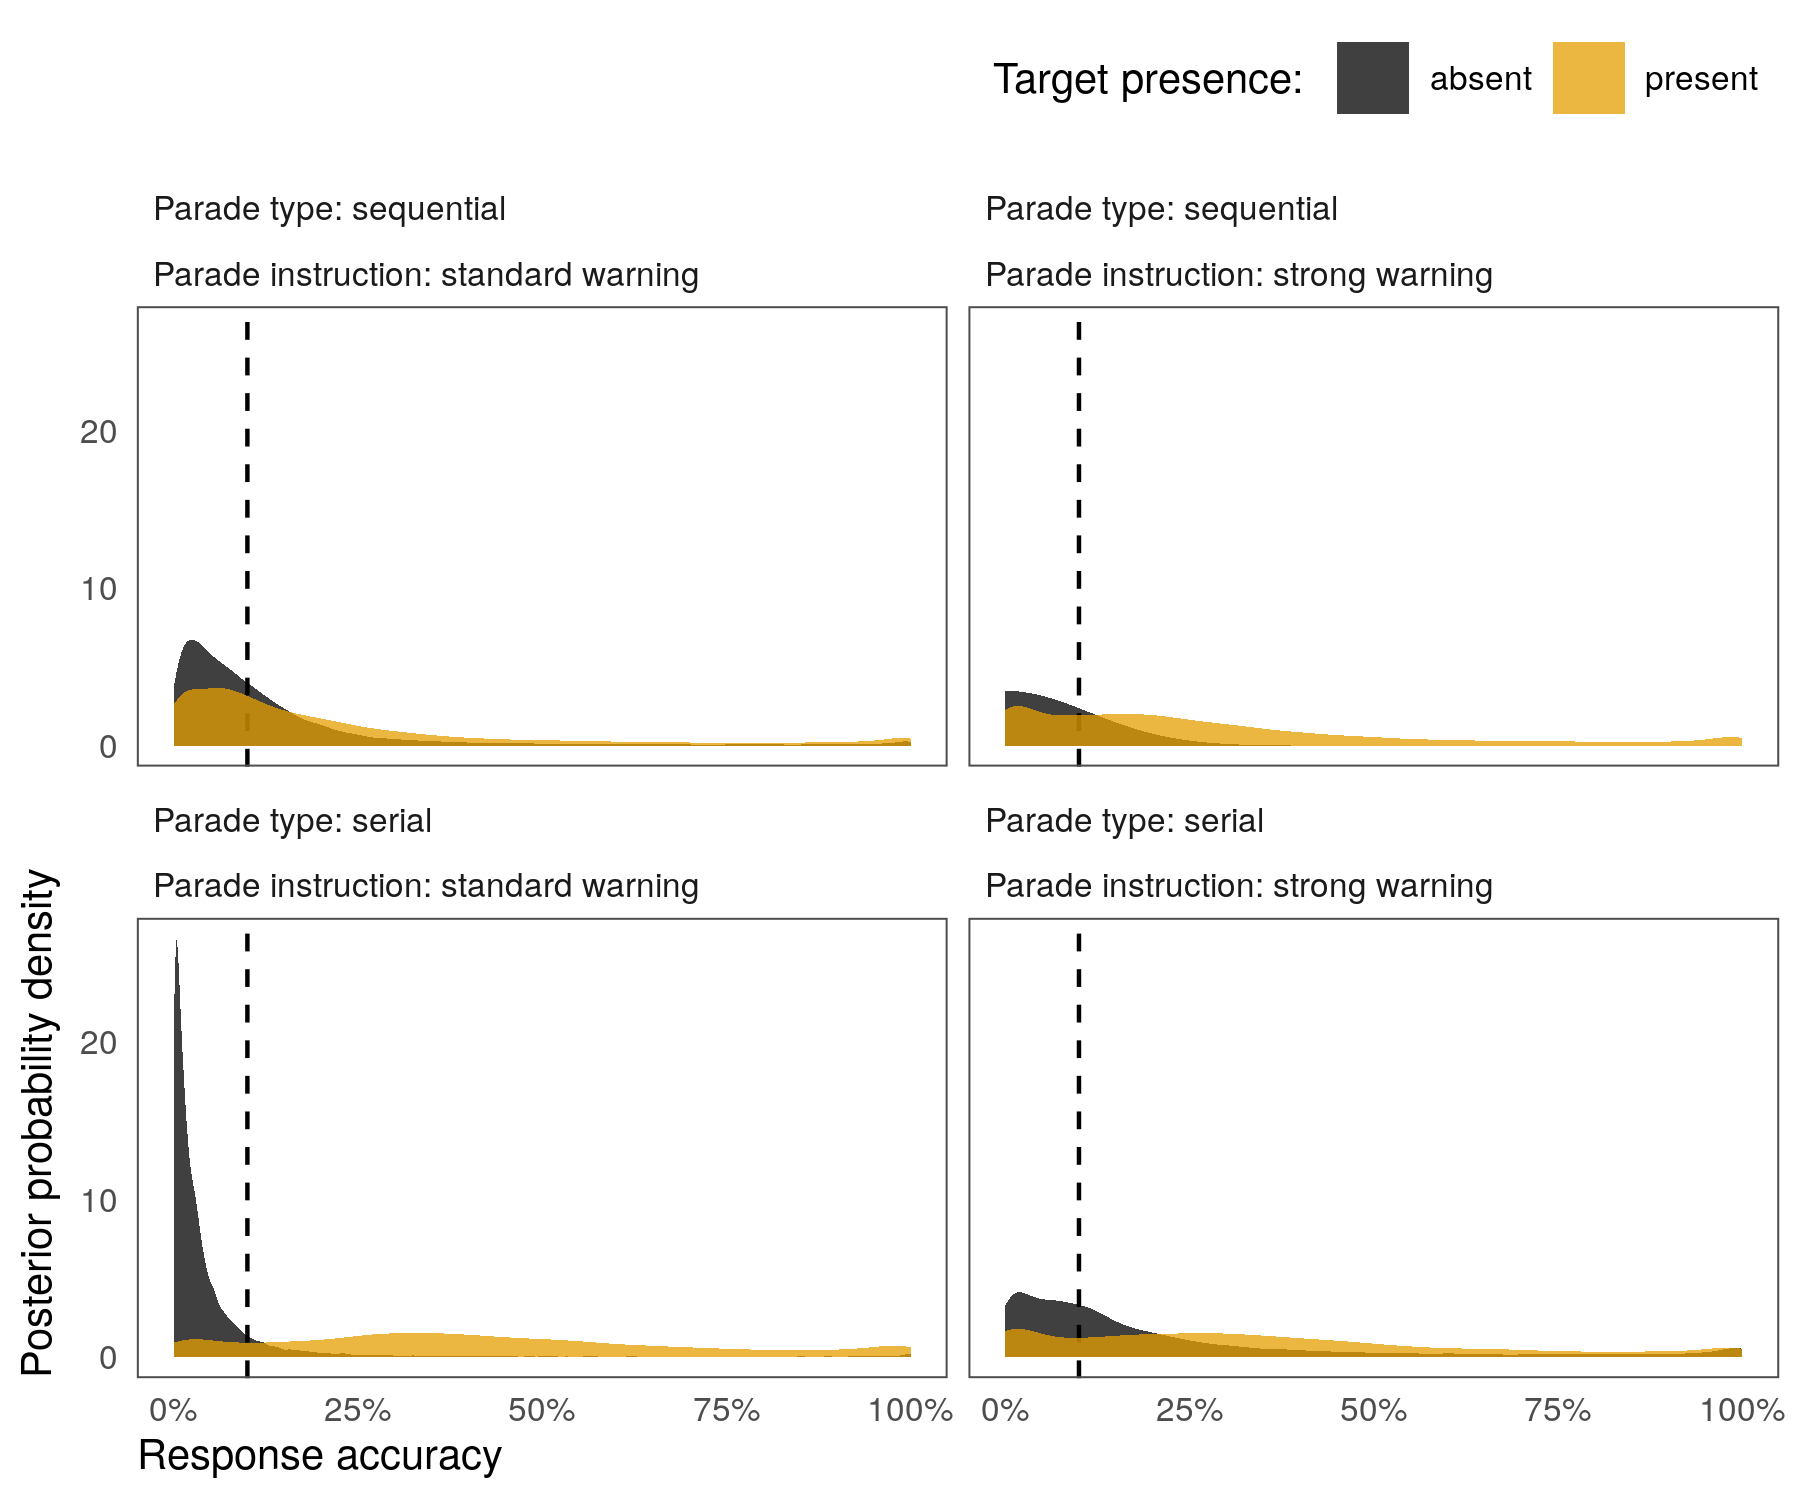
\includegraphics{../plots/online_probdist_byFA_L1} 

}

\caption{\label{fig:probdist2L1}The posterior probability density of the response accuracy for target absent and target present lineups displayed in grey and yellow, respectively for L1 English participants. The posterior probability is shown by Parade type $\times$ FA warning to illustrate the performance against chance-level (10\%). The dashed line indicates chance-level performance.}(\#fig:figL1)
\end{figure}

The results indicates a high probability of incorrect decisions with a
more diffuse probability density distribution in target present lineups
indicating a large uncertainty about the true parameter value. The
presence of the target voice in lineups lead to a higher accuracy of
\(\hat{\mu}\)=29.91\% (95\% HPDI {[}-1.94\%, 87.84\%{]}) for serial
parades when standard FA warnings were provided. This difference was
negligible for strong FA warnings (\(\hat{\mu}\)=1.48\%, 95\% HPDI
{[}-43.54\%, 86.60\%{]}). In sequential parades, target presence did not
substantially increase response accuracy neither when strong
(\(\hat{\mu}\)=1.75\%, 95\% HPDI {[}0\%, 91.52\%{]}) nor when standard
FA warnings (\(\hat{\mu}\)=0.54\%, 95\% HPDI {[}-22.47\%, 61\%{]}) were
provided.

Figure \ref{fig:probdist2L1} shows that for target absent trials we
observe a large amount of posterior probability mass either centered
around or concentrated below chance-level indicating a high probability
of incorrect identifications. From these distributions we inferred the
posterior probability of below chance-level response accuracies. The
resulting values are illustrated in Figure \ref{fig:prob_chanceL1}.

\begin{figure}[!ht]

{\centering 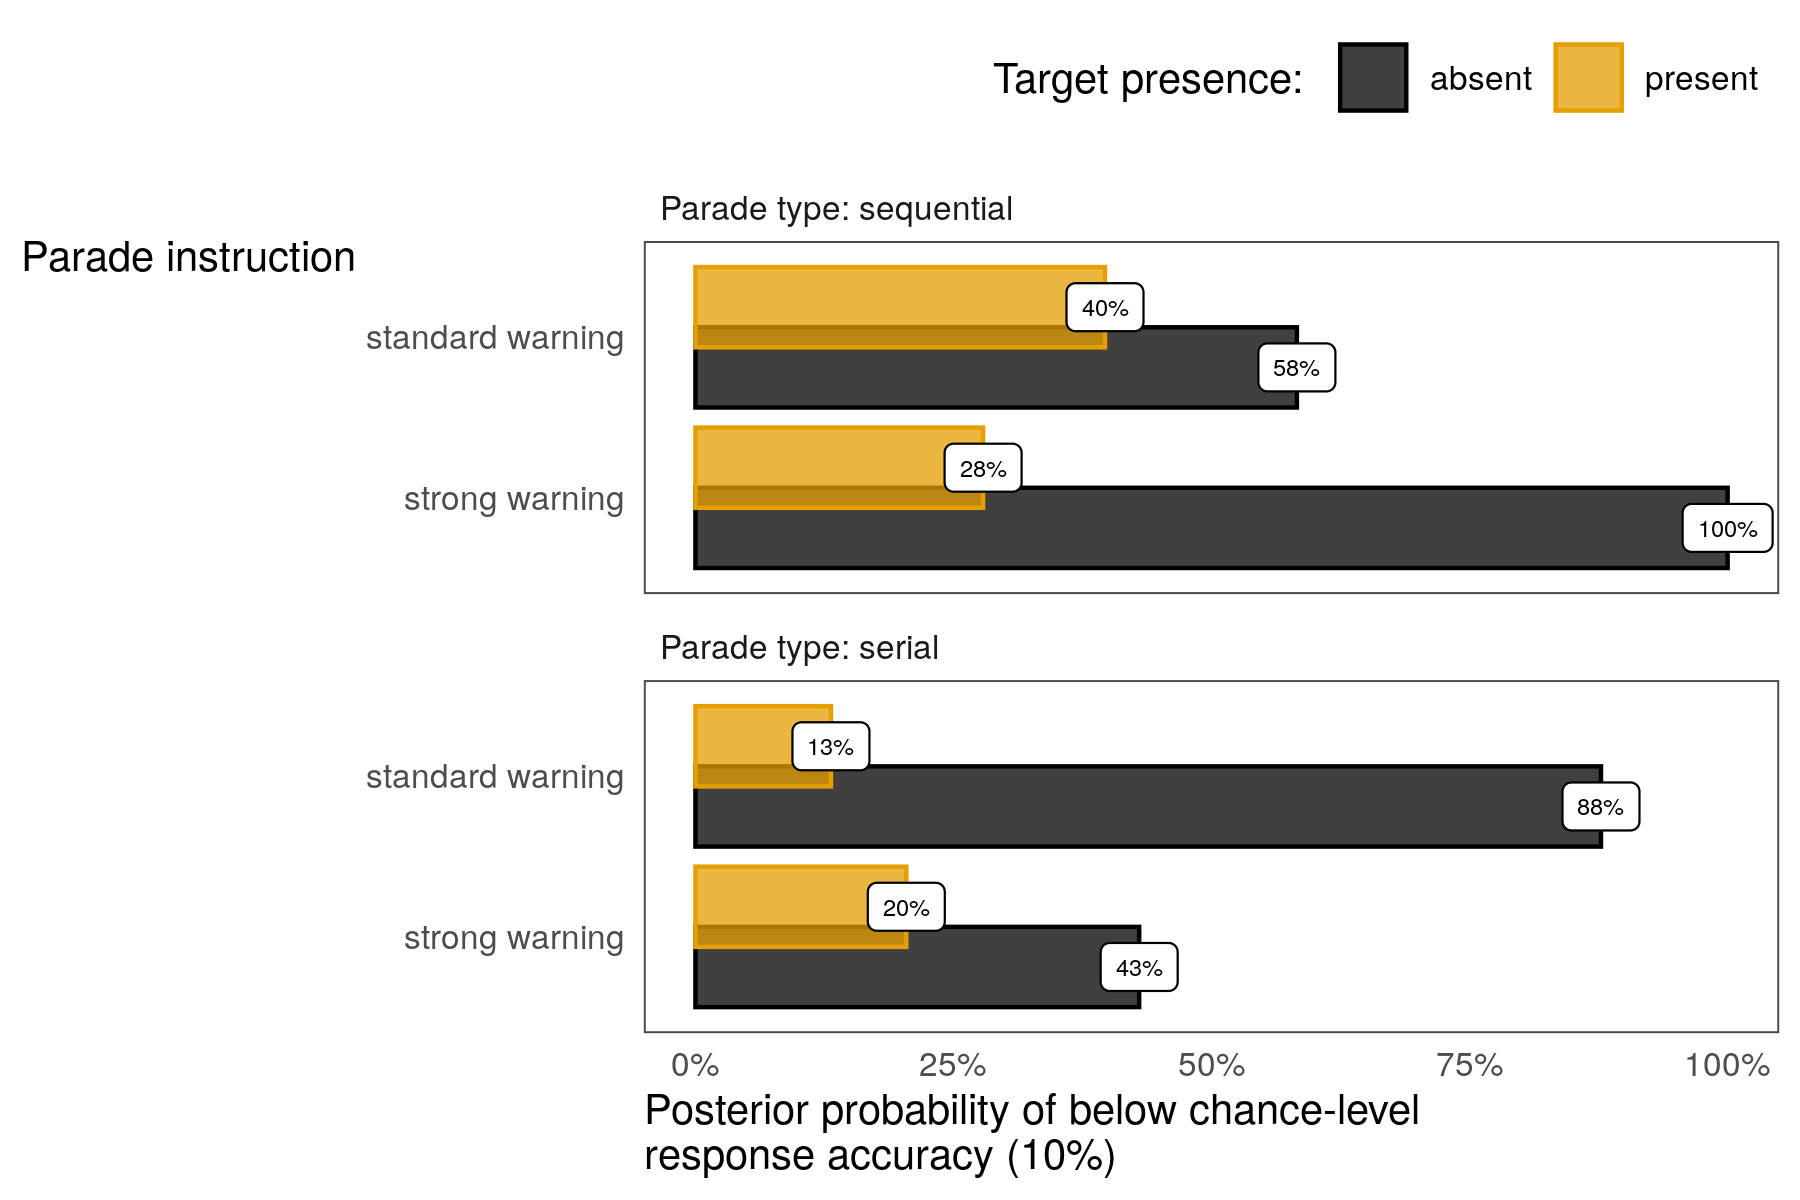
\includegraphics{../plots/prob_below_chance_L1} 

}

\caption{\label{fig:prob_chanceL1}The posterior probability of below chance-level (10\%) responses for target absent and target present lineups displayed in grey and yellow, respectively (L1 English participants).}(\#fig:figchanceL1)
\end{figure}

Figure \ref{fig:prob_chance} shows that target absent trials are
associated with a higher probability of below chance-level responses
compared to target present trials. The probability of below chance-level
responses was highest for target absent trials when strong FA warnings
were presented in sequential parades and for standard FA warnings in
serial parades. In particular, in serial parades the probability of
below chance-level responses was 44.74\% lower but 41.73\% higher in
sequential parades when strong FA warnings were provided. In other
words, FA warnings have opposite effects on the probability of observing
false-positives for serial compared to sequential parades. This
difference for target present lineups was substantially smaller,
i.e.~11.81\% for sequential parades and 7.30\% for serial parades.

\hypertarget{confidence-ratings}{%
\subsubsection{Confidence ratings}\label{confidence-ratings}}

Confidence ratings (0 - 10) were analysed in cumulative mixed effects
models for ordinal data. Accuracy was included as a nonlinear predictor
with adjustments for chance to prevent possible biases in the estimator.
The posterior ratings show an overall high confidence. There was no
evidence for any effects associated with response accuracy
(\(\hat{\mu}\)=1.96, 95\% PI {[}-3.13, 7{]}). The posterior confidence
ratings can be found in Table \ref{tab:confL1}. The evidence for
differences between conditions is negligible.

\begin{table}[h]

\begin{center}
\begin{threeparttable}

\caption{\label{tab:unnamed-chunk-8}\label{tab:confL1}L1 English participants. Posterior confidence ratings with
                  most probable parameter value and 95\% probability intervals in brackets for serial parades and sequential parades by factors Parade instruction (warning, no warning) and Target presence (present, absent).}

\begin{tabular}{llrr}
\toprule
Parade instruction & \multicolumn{1}{c}{Target presence} & \multicolumn{1}{c}{Parade type: sequential} & \multicolumn{1}{c}{Parade type:  serial}\\
\midrule
standard warning & absent & 7.97 [7.44, 8.39] & 7.93 [7.26, 8.44]\\
 & present & 8.03 [7.3, 8.54] & 7.9 [7.2, 8.46]\\
strong warning & absent & 8.02 [7.33, 8.51] & 7.78 [7.13, 8.37]\\
 & present & 8.1 [7.42, 8.57] & 7.58 [6.98, 8.27]\\
\bottomrule
\end{tabular}

\end{threeparttable}
\end{center}

\end{table}

\hypertarget{first-language}{%
\section{First language}\label{first-language}}

The response accuracy and confidence ratings might be affected by
whether or not the participant was a native speaker of English. To
account for this possibility we modelled the response accuracy and
confidence ratings in Bayesian models as described in the results
section. The predictor variable was L1 (1 = English, 0 = Others). Figure
\ref{fig:postL1} shows the outcome of both models. Figure
\ref{fig:postL1}a shows the posterior distribution of response
accuracies, indicating that response accuracy for other first languages
than English was distributed tighter around chance level. Figure
\ref{fig:postL1}b shows the confidence ratings as a function of response
accuracy by first language. The results show that participants with a
different first language than English responded with a slightly lower
confidence, in particular for incorrectly judged lineups. Overall there
is negligible evidence for systematic differences between native and
non-native speakers of English.

\begin{figure}[!ht]

{\centering 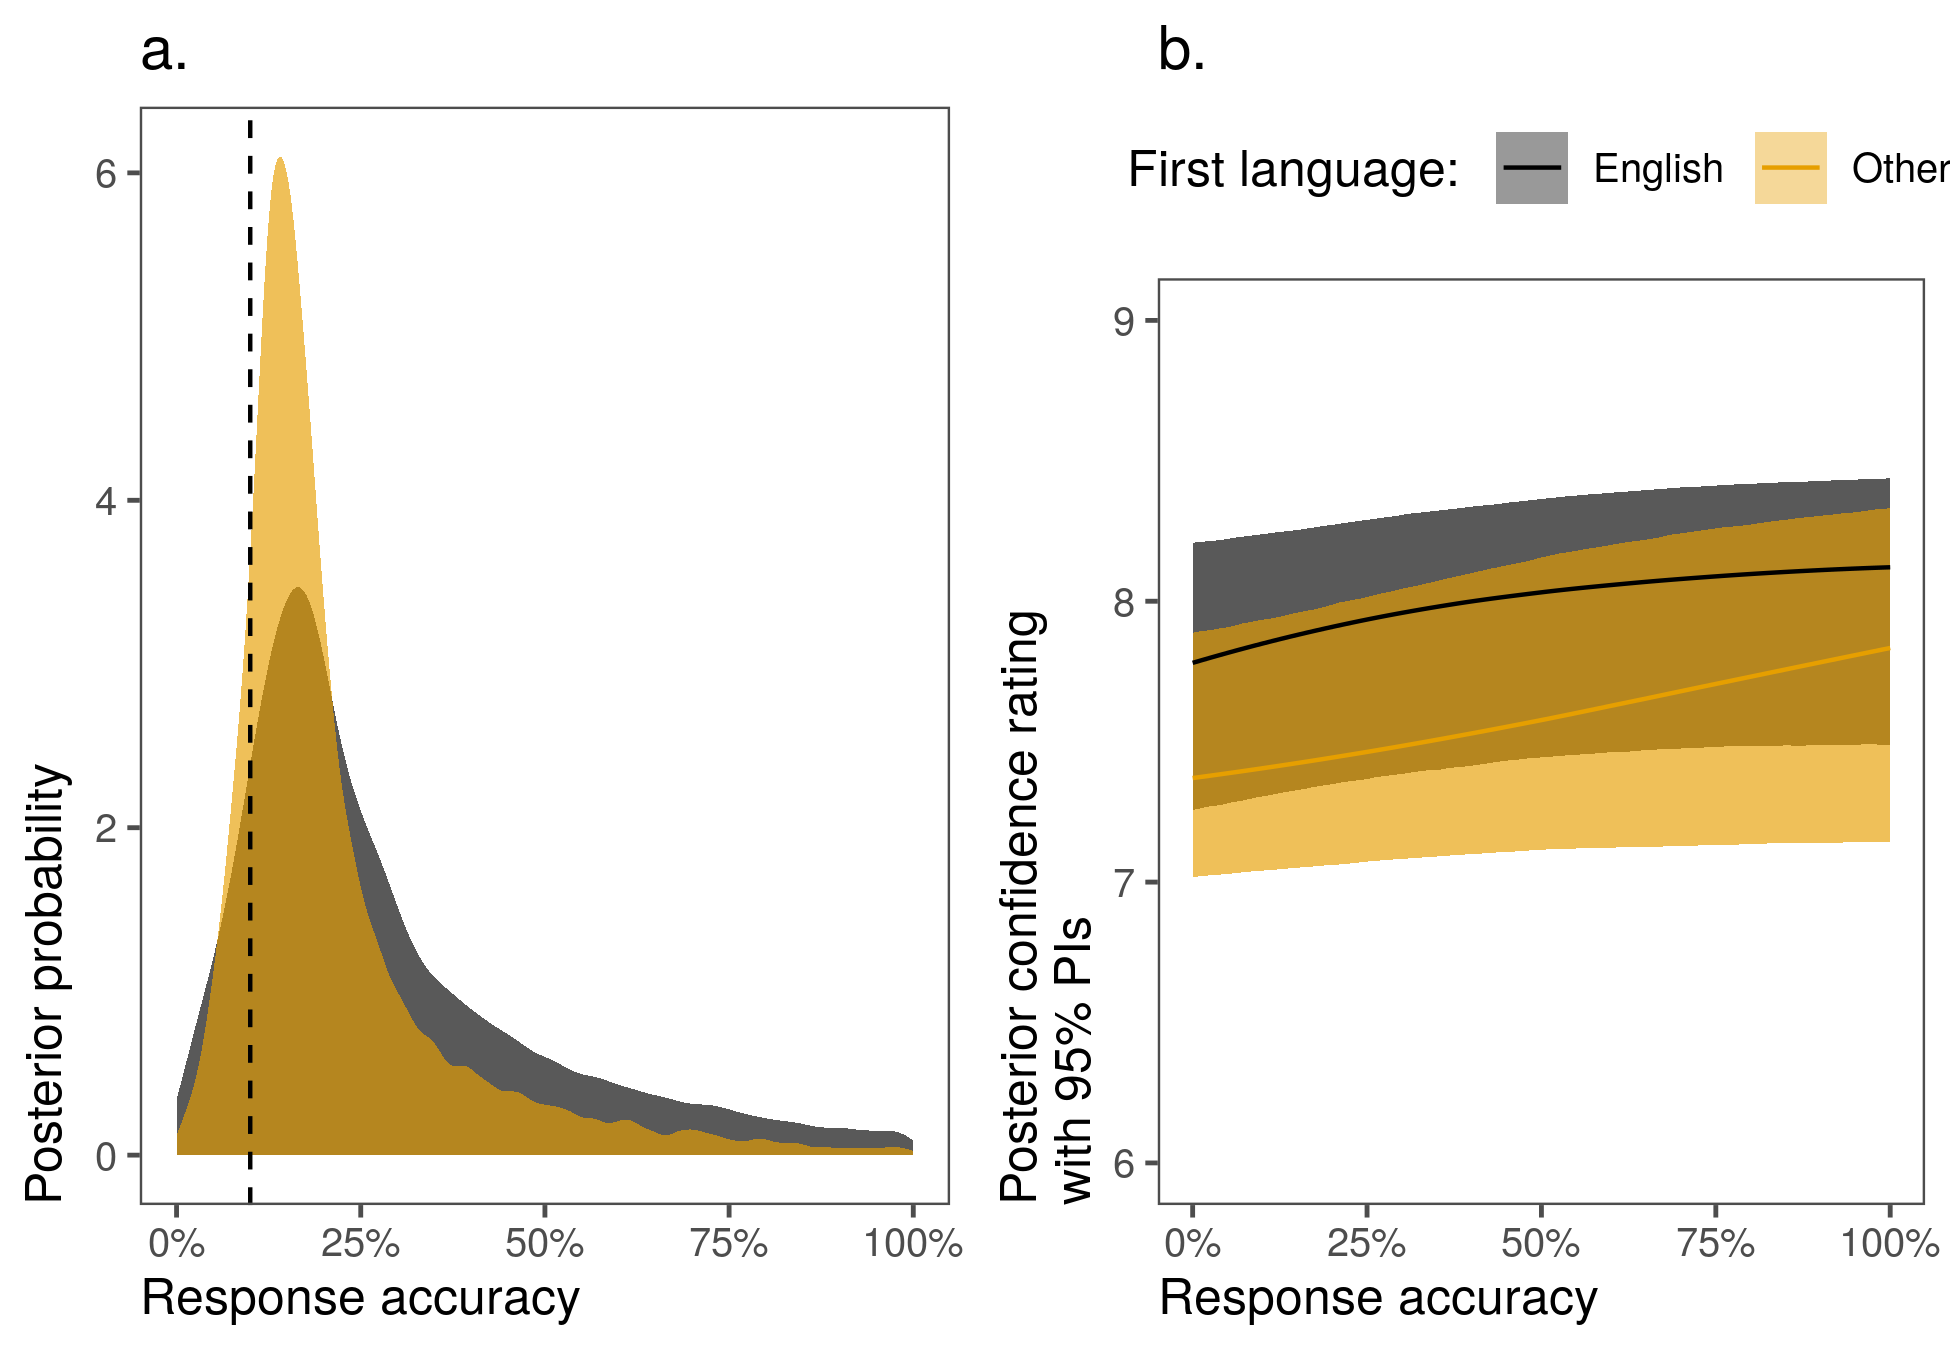
\includegraphics{report_files/figure-latex/figconfL1-1} 

}

\caption{\label{fig:postL1}Posterior distribution by first language. Panel (a) shows the distribution of the response accuracy relative to chance-level indicated by the dashed line. Panel (b) shows the confidence ratings as a function of response accuracy. The lines indicate $\hat{\mu}$, the most probable parameter value, and error ribbons show 95\% PIs.}(\#fig:figconfL1)
\end{figure}
\end{appendix}
